%%%%%%%%%%%%%%%%%%%%%%%%%%%%%%%%%%%%%%%%%%%%%%%%%%%%%%%%%%%%%%%%%%%%%%%%%%%%%%%%%
%%%%%                                RESULTS                                 %%%%
%%%%%%%%%%%%%%%%%%%%%%%%%%%%%%%%%%%%%%%%%%%%%%%%%%%%%%%%%%%%%%%%%%%%%%%%%%%%%%%%%

In this section we present our main results. In all cases standard errors are clustered at the 
state level so to match the main source of variation of the MW changes. We initially show how the 
estimated elasticity of rents to MW is approximately 0.025 when adopting the \textit{static DiD} 
model. We then present estimates for the \textit{dynamic} models that highlight both the absence 
of pre-trends, and the presence of a 2-months dynamic effect: the cumulative impact of a 10 \% MW 
change is estimated to be between 0.5 and 0.6 \% over the course of the 5 months after the policy 
change.

In \autoref{sec:sample_rest} we assess to what extent our results are representative of the true 
underlying Average Treatment Effect in two ways. First, since Zillow is present in relatively more 
dynamic markets than the average U.S. zipcode, we reweight observations so as to match population 
demographics for the top 100 CBSA. We show that the estimated impact slightly increases to 0.035 
\% indicating how our estimates can be seen as a lower bound. Second, we expand the panel used 
for the estimation by including zipcodes ``entering" after 2010. We control for changes in zipcode 
composition by contolling for \textit{entry cohort} $\times$ \textit{year-month} and we show how 
results are robust. We subsequently check for the presence of unobserved time-varying factors 
systematically affecting changes in MW and rents that may confound our estimates. We progressively 
include controls for the local economy, the labor and the housing market and we show how results 
do not change.

After establishing the robustness of our results, we then investigate how the incidence of the 
effect may vary across zipcodes. We use LODES data to proxy for MW workers residence and workplace 
location to show how effects disproportionately affect those zipcode that are more likely to have 
MW worker residents. We additionally estimate the heterogeneous impact of MW changes across the 
distribution of several census-based demographics. We show how effects are disproportionately 
concentrated in poorer, less-educated, and more African American zipcodes.


%%%%%%%%%%%%%%%%%%%%%%%%%%%%%%%%%%%%%%%%%%%%%%%%%%%%%%%%%%%%%%%%%%%%%%%%%%%%%%%%%
\subsection{Baseline Results}\label{sec:baseline_results}

In \autoref{tab:did_main}, we present results from the model defined in \autoref{eq:did}. In 
column 1, we show the classic two-way fixed effects (i.e. zipcode and year-month). To alleviate 
the concern that treated and untreated zipcodes could be on different time paths, in column 2 
(our baseline static DiD specification) we introduce linear time trends at the zipcode level. 
Finally, in column 3, we relax the linearity assumption on the zipcode-specific trends and allow 
for a quadratic time path for each zipcode. The estimated coefficients for MW changes are stable 
and significant across all specifications and indicate that a 10 percent increase in MW leads to 
a 0.26 percent increase in rent.

\begin{table}[h!]
    \caption{Results from Difference-in-Differences model}
    \label{tab:did_main}
    \centering
    {
\def\sym#1{\ifmmode^{#1}\else\(^{#1}\)\fi}
\begin{tabular}{l*{3}{c}}
\hline\hline
          &\multicolumn{1}{c}{(1)}&\multicolumn{1}{c}{(2)}&\multicolumn{1}{c}{(3)}\\
          &\multicolumn{1}{c}{D.ln\_med\_rent\_psqft}&\multicolumn{1}{c}{D.ln\_med\_rent\_psqft}&\multicolumn{1}{c}{D.ln\_med\_rent\_psqft}\\
\hline
D.ln\_mw   &   0.0257\sym{*}  &   0.0253\sym{**} &   0.0250\sym{**} \\
          & (0.0128)         & (0.0121)         & (0.0117)         \\
\hline
Zipcode-specifc linear trend&       No         &      Yes         &      Yes         \\
Zipcode-specific linear and square trend&       No         &       No         &      Yes         \\
R-squared &                  &                  &                  \\
Observations&    0.022         &    0.023         &    0.026         \\
N         &   113363         &   113363         &   113363         \\
\hline\hline
\end{tabular}
}

    \begin{minipage}{0.95\textwidth} \footnotesize
		\vspace{3mm} 
		\textit{Notes}: The table reports coefficients from versions of \autoref{eq:did} estimated 
		on the balanced panel of zipcode-months that contains SFCC rental price. Column (1) does not 
		include a zipcode-specific linear trend and results correspond to a two-way fixed effects 
		difference-in-differences. Column (2) includes zipcode-specific linear trends, and column (3) 
		allows for zipcode specific quadratic trends. Standard errors clustered at the state level. 
		*** $p < 0.01$, ** $p < 0.05$, * $p < 0.1$.
	\end{minipage}
\end{table}

In order to test for the presence of pre-trends in rents that may invalidate the causal 
interpretation of our results, we estimate the model with leads and lags of the MW changes defined 
in \autoref{eq:leads_lags}. We display the results in \autoref{tab:dynamic_lags_leads_main} and, 
again, present the results allowing progressively for more flexible zipcode level rental price 
heterogeneity over time.

\begin{table}[h!]
    \caption{Results from Difference-in-Differences model with leads and lags}
    \label{tab:dynamic_lags_leads_main}
    \centering
    {
\def\sym#1{\ifmmode^{#1}\else\(^{#1}\)\fi}
\begin{tabular}{l*{5}{c}}
\hline\hline
          &\multicolumn{1}{c}{(1)}         &\multicolumn{1}{c}{(2)}         &\multicolumn{1}{c}{(3)}         &\multicolumn{1}{c}{(4)}         &\multicolumn{1}{c}{(5)}         \\
\hline
$\Delta \ln \underline{w}_{ic,t-5}$&  -0.0148         &  -0.0144         &  -0.0144         &  -0.0146         &  -0.0144         \\
          & (0.0090)         & (0.0089)         & (0.0089)         & (0.0090)         & (0.0089)         \\
[1em]
$\Delta \ln \underline{w}_{ic,t-4}$&  -0.0024         &  -0.0019         &  -0.0020         &  -0.0022         &  -0.0019         \\
          & (0.0116)         & (0.0116)         & (0.0115)         & (0.0116)         & (0.0115)         \\
[1em]
$\Delta \ln \underline{w}_{ic,t-3}$&   0.0011         &   0.0005         &   0.0007         &   0.0004         &  -0.0002         \\
          & (0.0092)         & (0.0094)         & (0.0092)         & (0.0091)         & (0.0092)         \\
[1em]
$\Delta \ln \underline{w}_{ic,t-2}$&   0.0060         &   0.0063         &   0.0062         &   0.0060         &   0.0064         \\
          & (0.0116)         & (0.0118)         & (0.0116)         & (0.0115)         & (0.0117)         \\
[1em]
$\Delta \ln \underline{w}_{ic,t-1}$&  -0.0002         &  -0.0004         &  -0.0005         &   0.0000         &  -0.0005         \\
          & (0.0123)         & (0.0123)         & (0.0124)         & (0.0122)         & (0.0123)         \\
[1em]
$\Delta \ln \underline{w}_{ic,t}$&   0.0271\sym{**} &   0.0257\sym{**} &   0.0259\sym{**} &   0.0269\sym{**} &   0.0259\sym{**} \\
          & (0.0126)         & (0.0123)         & (0.0124)         & (0.0126)         & (0.0124)         \\
[1em]
$\Delta \ln \underline{w}_{ic,t+1}$&   0.0136\sym{*}  &   0.0146\sym{**} &   0.0142\sym{*}  &   0.0135\sym{*}  &   0.0146\sym{*}  \\
          & (0.0072)         & (0.0072)         & (0.0072)         & (0.0072)         & (0.0072)         \\
[1em]
$\Delta \ln \underline{w}_{ic,t+2}$&  -0.0070         &  -0.0066         &  -0.0064         &  -0.0068         &  -0.0064         \\
          & (0.0133)         & (0.0133)         & (0.0132)         & (0.0133)         & (0.0132)         \\
[1em]
$\Delta \ln \underline{w}_{ic,t+3}$&   0.0036         &   0.0045         &   0.0047         &   0.0031         &   0.0040         \\
          & (0.0081)         & (0.0078)         & (0.0078)         & (0.0079)         & (0.0077)         \\
[1em]
$\Delta \ln \underline{w}_{ic,t+4}$&   0.0108         &   0.0093         &   0.0104         &   0.0107         &   0.0096         \\
          & (0.0069)         & (0.0066)         & (0.0064)         & (0.0069)         & (0.0065)         \\
[1em]
$\Delta \ln \underline{w}_{ic,t+5}$&   0.0086         &   0.0095         &   0.0099         &   0.0088         &   0.0099         \\
          & (0.0069)         & (0.0065)         & (0.0065)         & (0.0067)         & (0.0065)         \\
\hline
\vspace{-2mm}&                  &                  &                  &                  &                  \\
Cumulative effect&    0.057         &0.057\sym{*}         &0.059\sym{*}         &    0.056         &0.058\sym{*}         \\
          &  (0.035)         &  (0.034)         &  (0.034)         &  (0.034)         &  (0.034)         \\
\hline    &                  &                  &                  &                  &                  \\
P-value no pretrends&    0.568         &    0.612         &    0.599         &    0.594         &    0.629         \\
Wage controls&       No         &      Yes         &       No         &       No         &      Yes         \\
Employment controls&       No         &       No         &      Yes         &       No         &      Yes         \\
Establishment-count controls&       No         &       No         &       No         &      Yes         &      Yes         \\
R-squared &    0.022         &    0.022         &    0.022         &    0.022         &    0.022         \\
Observations&  106,446         &  105,463         &  105,463         &  106,160         &  105,463         \\
\hline\hline
\end{tabular}
}

    \begin{minipage}{0.95\textwidth} \footnotesize
		\vspace{3mm} 
		\textit{Notes}: The table reports coefficients from versions of \autoref{eq:leads_lags} 
		estimated on the balanced panel of zipcode-months that contains SFCC rental price. Column 
		(1) does not include a zipcode-specific linear trend and results correspond to a two-way fixed-effects difference-in-differences. Column (2) includes zipcode-specific linear trends, 
		and column (3) allows for zipcode specific quadratic trends. Standard errors clustered at 
		the state level. *** $p < 0.01$, ** $p < 0.05$, * $p < 0.1$.
	\end{minipage}
\end{table}

Consistent with a causal interpretation of our results, future MW changes do not have an effect on 
rent prices. This suggests how there are no pre-treatment differentials in the evolution of rental 
prices between treated and untreated zipcodes. \autoref{tab:dynamic_lags_leads_main} additionally 
reports the results of an F-test for all leads to be jointly equal to zero. We comfortably fail to 
reject that hypothesis in all cases. On the other hand, we detect a significant effect on rents at 
the period of the MW change. Specifically, we estimate that rents increase by around 0.27 percent 
following a $10$ percent raise in the MW (column 2), and the effect is largely unchanged both by the 
exclusion of linear trends (column 1) and by the inclusion of more flexible zipcode quadratic level 
trends (column 3).

A second important result shown by \autoref{tab:dynamic_lags_leads_main} is the presence of a mild 
persistence of the effect of MW changes on rents. After a 10 percent change in the MW, rents tend to 
increase by $0.13$ percent in the month \textit{after} the change, while the impact appears to vanish 
after the first two periods. In column 3 the estimated coefficients in $t+1$ loses statistical 
significance being slightly lower, but the point estimate remains larger than any of the following 
post-treatment periods. The results shown implies that - when allowing for dynamic effects of MW 
changes on rents - the cumulative impact is even larger than the one estimated by the static DiD 
model. Over the course of a semester, a $10$ percent raise in the MW translates to between $0.5$ 
and $0.6$ percent increase in the rental price.

\begin{figure}
    \caption{Estimated Impact of changes in MW on changes in Rents for Different Specifications}
    \label{fig:fd_models_main}
    \centering
    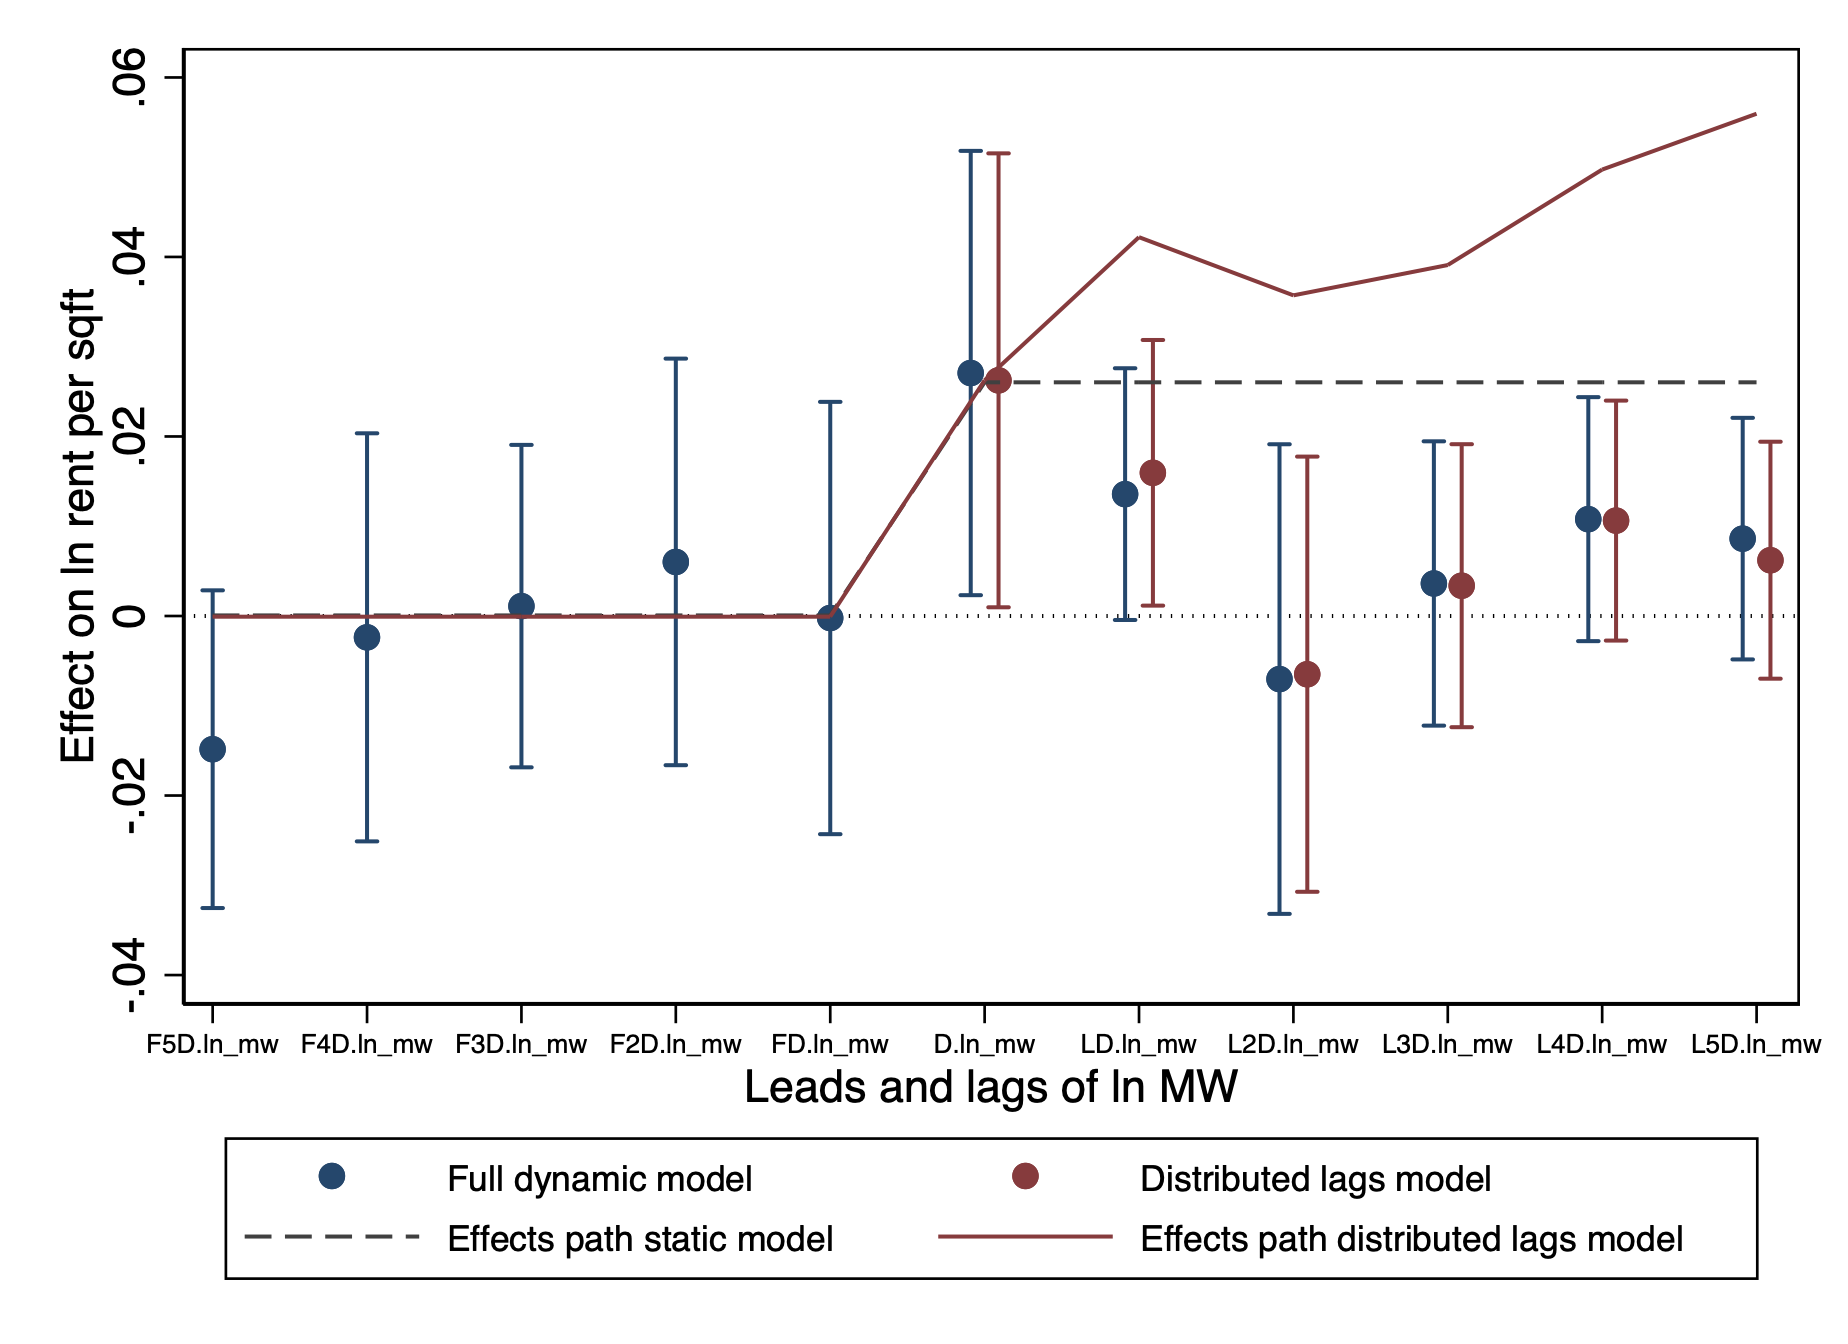
\includegraphics[width = 0.8\textwidth]{../analysis/first_differences/output/fd_models.png}
    \begin{minipage}{0.95\textwidth} \footnotesize
		\vspace{2mm} 
		\textit{Notes}: The plot shows the estimated coefficients for the \textit{dynamic DiD} 
		models estimated through \autoref{eq:leads_lags} and (\ref{eq:lags}) alongside 90 percent 
		confidence intervals. The dashed line additionally reports the point estimate from the 
		\autoref{eq:did}. The solid red line show the point estimates for the cumulative effects 
		estimated through the distributed lags model in \autoref{eq:lags}. Standard errors for both 
		the \textit{static} and the final period of the distributed lag models are reported in 
		\autoref{tab:did_main} and \autoref{tab:dynamic_cumulative} respectively. 
	\end{minipage}
\end{figure}

We summarize and compare the results from the \textit{static} and the \textit{dynamic} DiD models 
in \autoref{fig:fd_models_main}. The dashed line shows the effect path on rents implied by the 
point estimates (the standard error is omitted to avoid cluttering the figure) from the static DiD 
(equation \ref{eq:did}). The blue-dot series plots the estimates from \autoref{eq:leads_lags}, where 
we can appreciate the absence of pre-trends and that the bulk of the effect is concentrated in the 
first two periods. We also report the estimated coefficients from the dynamic model defined in 
\autoref{eq:lags} (red-dot series), showing how the estimates mimic closely those found with the 
leads and lags model. Finally, with the continuous red line we show the cumulative effect of MW 
changes on rents implied by the red dots. As stated before, the effects implied by the dynamic models 
are larger than the ones implied by the static DiD.

To directly account for the presence of zipcode level rent dynamics, we further test our results by 
estimating a \textit{dynamic} DiD model that controls for the lagged value of the changes in rents 
(equation \ref{eq:ab_panel}). We compare that with our baseline estimates in 
\autoref{tab:horse_race_main}: columns 1, 2, and 3 show coefficients from equations \eqref{eq:did}, 
\eqref{eq:leads_lags}, and \eqref{eq:lags} respectively. In columns 4 and 5, we allow for full blown 
dynamics in the dependent variable and we recover the coefficients using instrumental variables 
following the classic \textcite{arellano1991some} approach --using deeper lags of the dependent 
variable to instrument for the lagged dependent variable-- for the cases with and without leads. 
In columns 6 and 7 we show estimates from the model in equation \ref{eq:ab_panel} but instrumenting 
the lagged dependent variable with the sixth MW change lag as in \textcite{meer2016effects}. Our 
effects are robust to all of this stringent tests: the same-month change in rents following a 10 
percent increase in MW is consistently estimated between 0.25 and 0.3 percent. 


\subsection{External Validity and Data Sensitivity}\label{sec:sample_rest}

Our results suggest a noticeable impact of MW policies on the rental housing market. However, as 
explained in \autoref{sec:data}, the number of zipcodes included in the final sample is only a 
small portion of the total U.S., and they come from more urban and richer neighborhoods that likely 
have a dynamic housing market. This limited sample size might hinder the external validity of the 
estimated effect. Additionally, the zipcodes included in the final sample are the ones appearing 
earlier in the Zillow data (i.e. zipcodes whose rent data are available since January 2010), and 
this might result in unobserved differences affecting sample selection.

We test the sensitivity with respect to our sample restrictions in two ways. First, we extend our 
panel by including the full set of zipcodes for which there is available rent data. This, on one 
hand, doubles the sample size (we now use the full $3,316$ zipcode in the Zillow rent data for 
single family, condos and cooperative houses), but, on the other hand, makes the composition of 
zipcodes vary over time by including, as they enter the sample, zipcodes whose time series start 
later than January 2010. Therefore, to fully exploit our data we estimate models using an unbalanced 
panel but controlling for ``cohort $\times$ period" fixed effects. We do this for our main 
specifications in equations \eqref{eq:did}, \eqref{eq:leads_lags}, and \eqref{eq:lags}. In this way, 
we are able to compare treated and untreated zipcodes with the same panel length. In 
\autoref{tab:comparison_unbal_base} we show that that the estimated effects for the different models 
remain widely unchanged. In \autoref{fig:dynamic_dd_comparison}, panel (a) we compare 
\textit{dynamic} DiD estimates obtained using the baseline sample and the unbalanced sample. Using 
the unbalanced panel, our estimates are slightly lower but they are largely identical to the baseline 
results.

Secondly, we assess the representativeness of our estimates by re-weighting zipcodes so as to match 
socio-demographic characteristics of the zipcodes in the top-100 CBSA. We do this by applying the 
entropy balancing procedure developed by \cite{hainmueller2012entropy} on the following zipcode 
level demographics: share of rental houses, share of African-American residents, share of college 
graduates, and median income. We target averages from \autoref{tab:desc_stats}, column 
2.\footnote{The entropy balancing procedure consists of a re-weighting scheme that assigns a scalar 
	weight to every unit such that the re-weighted sample matches moments of a target population. We 
	implement this by leveraging the \texttt{STATA} package \texttt{ebalance} described in 
	\textcite{hainmueller2013ebalance}.} 
We subsequently re-estimate our models with weighted regressions.

The results shown in \autoref{fig:dynamic_dd_comparison}, panel(b) confirm what we found in our 
baseline case, although point estimates are somewhat higher. Note that the simultaneous effect from 
the \textit{dynamic} DiD model presents the only statistically significant post-treatment 
coefficient. The effect in month $t+1$ becomes indeed smaller and not significant, suggesting how 
the baseline model might overestimate the persistence of the true average effect. A comparison with 
the \textit{static} DiD estimate supports this finding: $\hat{\beta}$ from \autoref{eq:did} and 
$\hat{\beta}_{t}$ from \autoref{eq:leads_lags} are almost identical, identifying an elasticity on 
rents of approximately $0.036$ (\autoref{tab:comparison_wgt_base}).

\begin{figure}[htb!]
    \caption{Comparison between dynamic DiD models}
    \label{fig:dynamic_dd_comparison}
    \centering
    \begin{subfigure}[b]{0.8\textwidth}
        \caption{Unbalanced panel}
        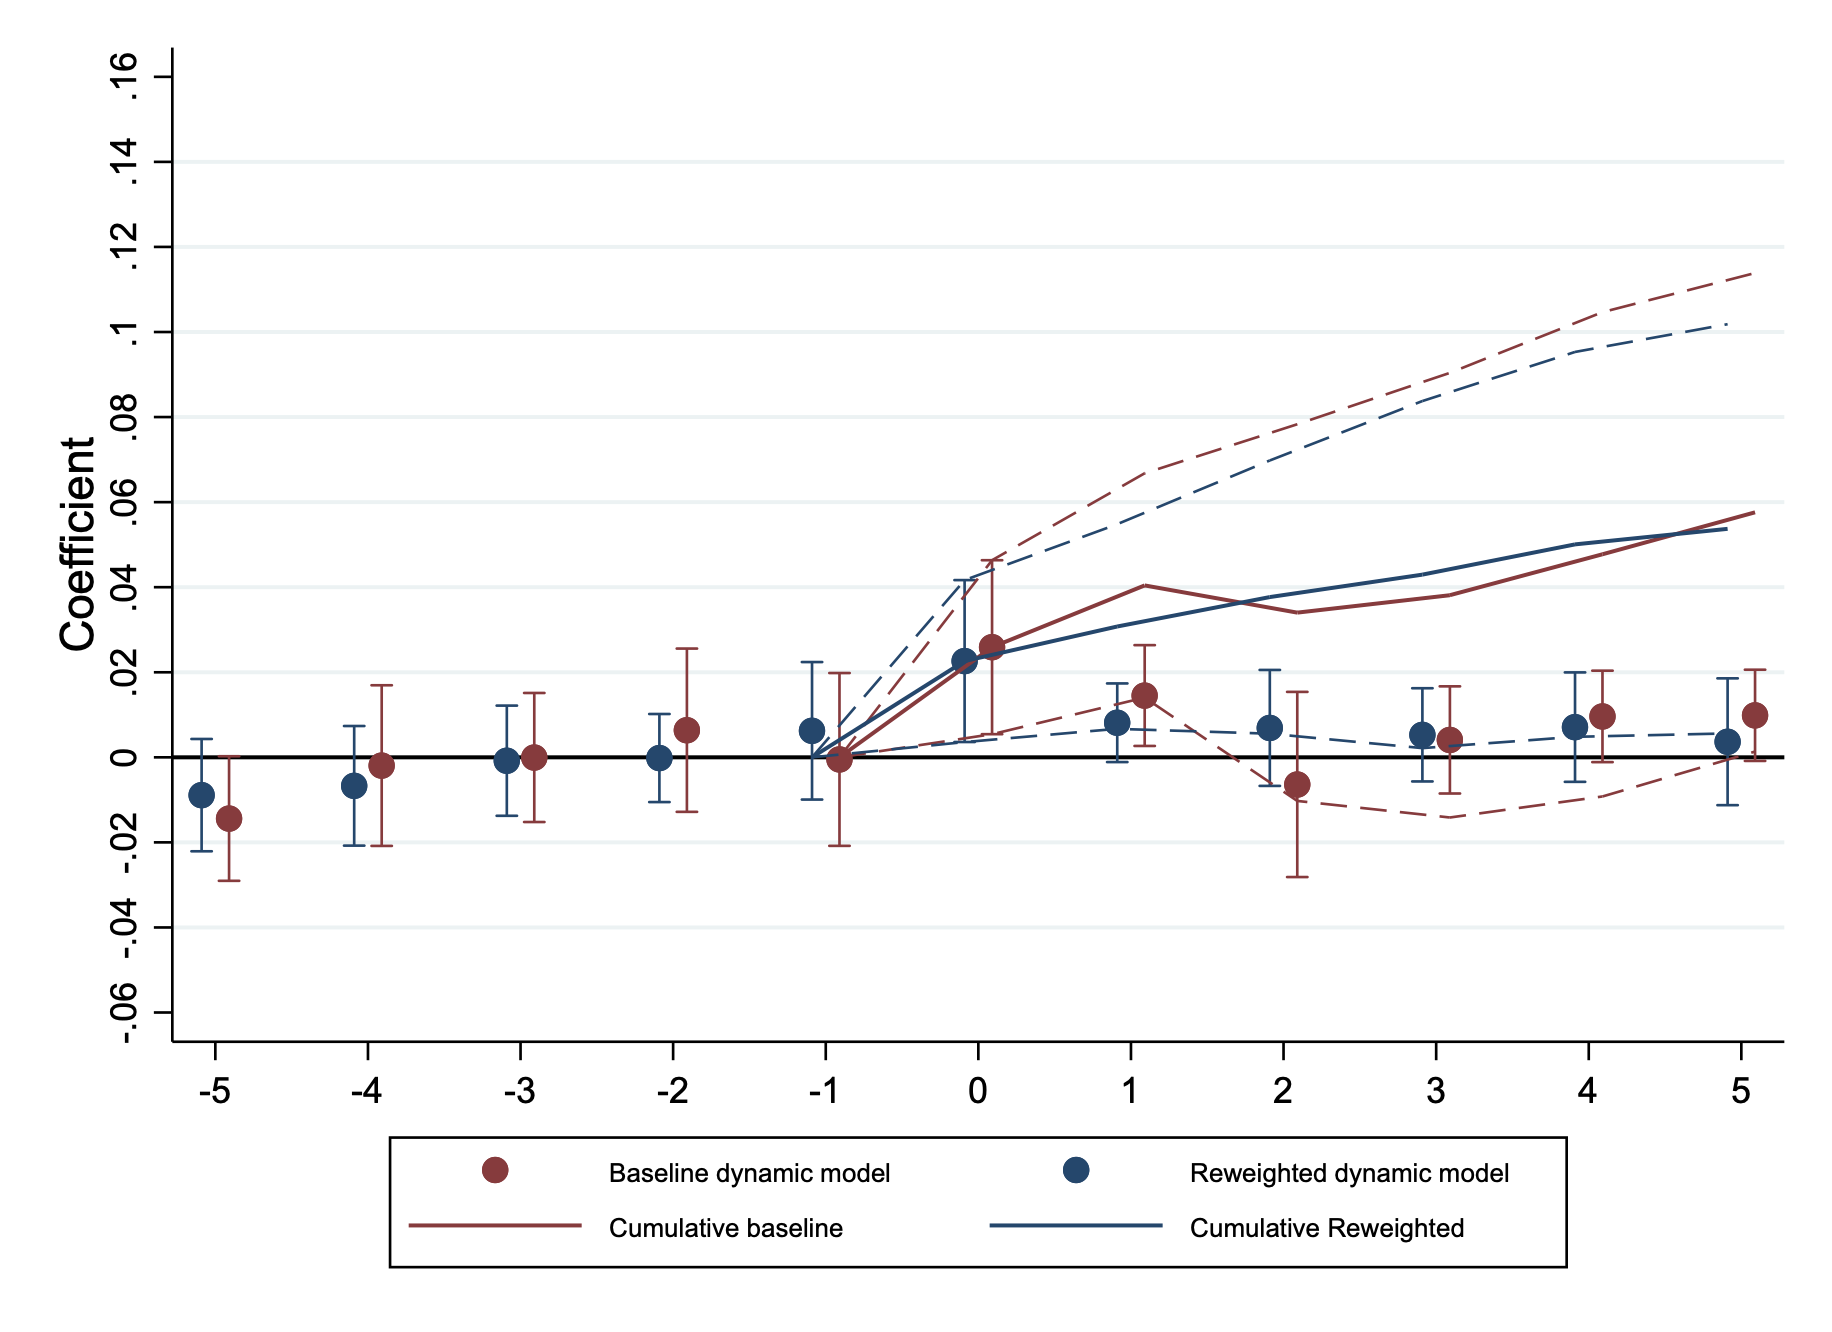
\includegraphics[width = \textwidth]
        {../analysis/first_differences_unbal/output/fd_model_comparison_unbal.png}
    \end{subfigure}
    \begin{subfigure}[b]{0.8\textwidth}
        \caption{Reweighted panel}
        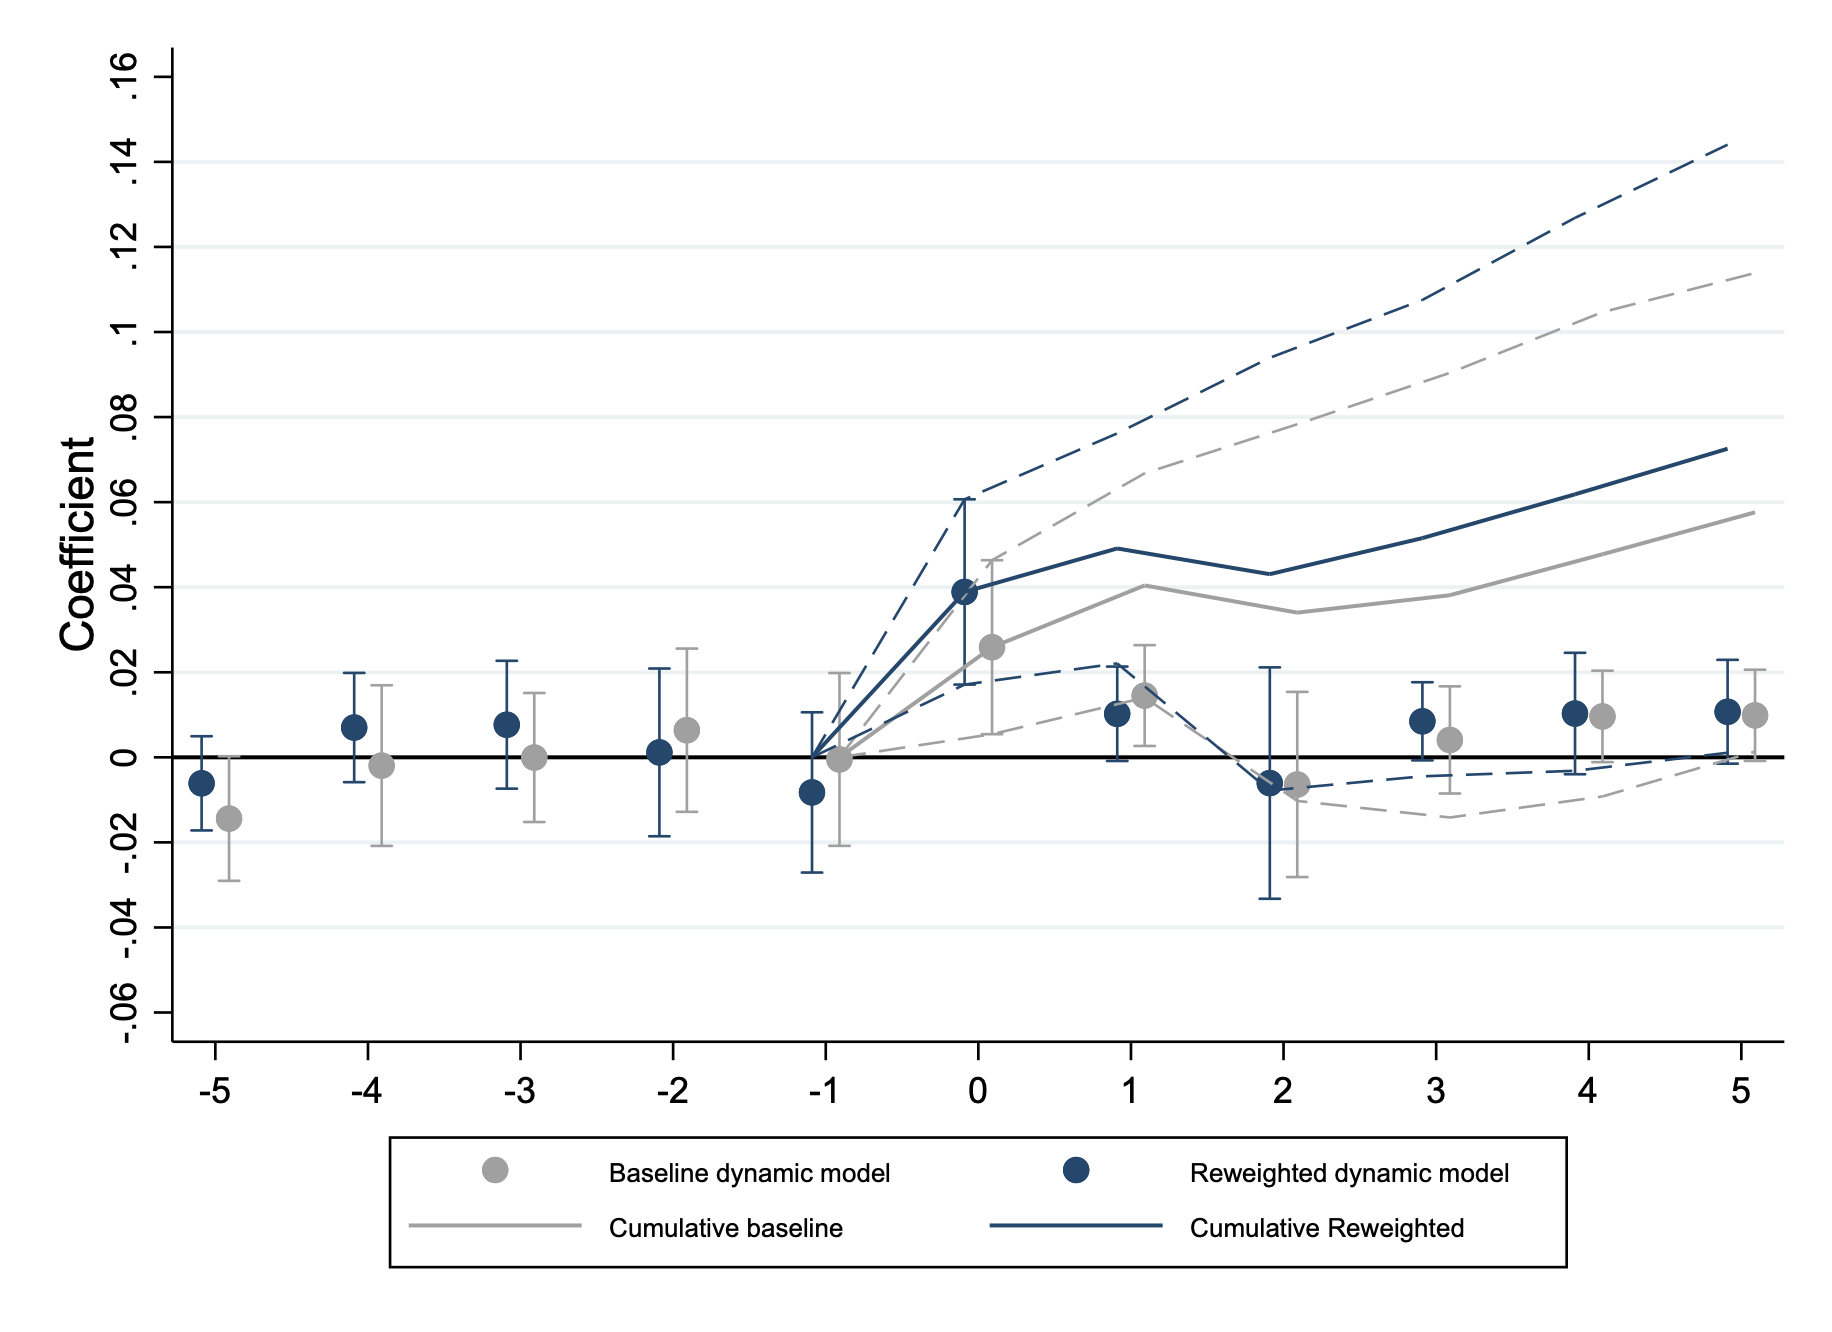
\includegraphics[width = \textwidth]
        {../analysis/first_differences_wgt/output/fd_model_comparison_wgt.png}
    \end{subfigure}
    \begin{minipage}{0.95\textwidth} \footnotesize
		\vspace{2mm} 
		\textit{Notes}: The plot compares results obtained from the baseline panel summarized in 
		\autoref{tab:desc_stats}, column 4 with those obtained from the full unbalanced panel (a), 
		and with the reweighted baseline panel (b). Each subfigure compares estimated coefficients 
		for the \textit{dynamic DiD} models calculated through \autoref{eq:leads_lags}, and point 
		estimates for the cumulative effect of MW on rents estimated through \autoref{eq:lags}.   
	\end{minipage}
\end{figure}


%%%%%%%%%%%%%%%%%%%%%%%%%%%%%%%%%%%%%%%%%%%%%%%%%%%%%%%%%%%%%%%%%%%%%%%%%%%%%%%%%
\subsection{The Role of Unobserved Local Shocks}\label{sec:econ_shocks}

In \autoref{sec:baseline_results} we used \autoref{eq:leads_lags} to establish the absence of 
significant pre-trends in rent dynamics. Another potential threat to the identification of the true 
causal effect might come from unobserved local shocks systematically affecting MW and rent changes. 
In order to account for that, we directly control for proxies of general economic shocks, as well as 
shocks related to the labor and housing markets aggregated at either the county-month or 
county-quarter level, while rents are defined at the zipcode-level. While this prevents us from 
studying the presence of zipcode-level time-varying confounding factors, it substantially strengthens 
the robustness of the estimated impact since the treatment is administered at city, county, or state 
level. In fact, if there are underlying factors affecting MW changes that also affect zipcode-level 
rents, they would likely arise from this larger geographic units.

Controls included in our regressions are the following. First, to account for local economic shocks, 
we use the county-quarter number of establishments by industry obtained from the QCEW (see 
\autoref{sec:data} for more details). We then proxy for local labor market dynamics with two sets 
of controls: county-quarter weekly average wage, and county-month employment by industry. Since we 
are using a first-difference specification, we augment each model with their log difference. Second, 
we proxy for shocks that may stem from the housing market using the county-month number of new 
permits for residential one-unit buildings and the associated permits' valuation. Since these two 
series already report changes between periods, we only control for the log levels.

\begin{table}[h!]
    \caption{Results from Difference-in-Differences model with leads and lags and controls}
    \label{tab:dynamic_leads_lags_econshock}
    \centering
    \resizebox{0.9\textwidth}{!}{
	    \vspace{0pt}
	    {
\def\sym#1{\ifmmode^{#1}\else\(^{#1}\)\fi}
\begin{tabular}{l*{5}{c}}
\hline\hline
          &\multicolumn{1}{c}{(1)}&\multicolumn{1}{c}{(2)}&\multicolumn{1}{c}{(3)}&\multicolumn{1}{c}{(4)}&\multicolumn{1}{c}{(5)}\\
          &\multicolumn{1}{c}{D.ln\_med\_rent\_psqft}&\multicolumn{1}{c}{D.ln\_med\_rent\_psqft}&\multicolumn{1}{c}{D.ln\_med\_rent\_psqft}&\multicolumn{1}{c}{D.ln\_med\_rent\_psqft}&\multicolumn{1}{c}{D.ln\_med\_rent\_psqft}\\
\hline
F5D.ln\_mw &  -0.0157         &  -0.0150\sym{*}  &  -0.0150\sym{*}  &  -0.0146\sym{*}  &  -0.0191\sym{*}  \\
          &(0.00938)         &(0.00832)         &(0.00816)         &(0.00823)         &(0.00983)         \\
[1em]
F4D.ln\_mw & -0.00382         & -0.00125         & -0.00131         & -0.00114         & -0.00776         \\
          & (0.0101)         &(0.00874)         &(0.00875)         &(0.00873)         &(0.00938)         \\
[1em]
F3D.ln\_mw &-0.000214         & -0.00150         & -0.00179         & -0.00133         &  0.00420         \\
          &(0.00831)         &(0.00889)         &(0.00910)         &(0.00885)         &(0.00917)         \\
[1em]
F2D.ln\_mw &  0.00477         &  0.00200         &  0.00219         &  0.00263         &  0.00276         \\
          & (0.0115)         & (0.0115)         & (0.0116)         & (0.0117)         & (0.0133)         \\
[1em]
FD.ln\_mw  & -0.00143         & -0.00398         & -0.00397         & -0.00394         &  -0.0114         \\
          & (0.0142)         & (0.0146)         & (0.0145)         & (0.0145)         & (0.0167)         \\
[1em]
D.ln\_mw   &   0.0260\sym{**} &   0.0265\sym{**} &   0.0269\sym{**} &   0.0258\sym{**} &   0.0267\sym{*}  \\
          & (0.0110)         & (0.0113)         & (0.0108)         & (0.0105)         & (0.0140)         \\
[1em]
LD.ln\_mw  &   0.0118         &   0.0108         &   0.0112         &   0.0115         &   0.0169\sym{**} \\
          &(0.00805)         &(0.00834)         &(0.00859)         &(0.00878)         &(0.00752)         \\
[1em]
L2D.ln\_mw & -0.00884         & -0.00554         & -0.00561         & -0.00548         & -0.00101         \\
          & (0.0124)         & (0.0126)         & (0.0127)         & (0.0127)         & (0.0143)         \\
[1em]
L3D.ln\_mw &  0.00191         &  0.00324         &  0.00326         &  0.00453         &  0.00845         \\
          &(0.00812)         &(0.00821)         &(0.00829)         &(0.00795)         &(0.00837)         \\
[1em]
L4D.ln\_mw &  0.00918         &   0.0105         &   0.0108         &  0.00968         &   0.0105         \\
          &(0.00724)         &(0.00686)         &(0.00680)         &(0.00683)         &(0.00675)         \\
[1em]
L5D.ln\_mw &  0.00736         &  0.00743         &  0.00749         &  0.00748         &  0.00702         \\
          &(0.00717)         &(0.00785)         &(0.00782)         &(0.00775)         &(0.00834)         \\
\hline
P-value no pretrends&    0.602         &    0.632         &    0.609         &    0.633         &    0.514         \\
Industry-level monthly employment&       No         &      Yes         &      Yes         &      Yes         &      Yes         \\
Industry-level quarterly establishment count&       No         &       No         &      Yes         &      Yes         &      Yes         \\
Industry-level quarterly weekly wage&       No         &       No         &       No         &      Yes         &      Yes         \\
New housing permits and value&       No         &       No         &       No         &       No         &      Yes         \\
R-squared &    0.027         &    0.028         &    0.028         &    0.028         &    0.031         \\
Observations&   106446         &   101448         &   101448         &   101448         &    82716         \\
\hline\hline
\end{tabular}
}
}
    \begin{minipage}{0.95\textwidth} \footnotesize
		\vspace{3mm} 
		\textit{Notes}: The table reports coefficients from \autoref{eq:leads_lags} estimated on the 
		balanced panel of zipcode-months that contains SFCC rental price. All specifications include 
		zipcode linear trends. Column (1) replicates our baseline results from 
		\autoref{tab:dynamic_lags_leads_main}, column 2. Columns 2 to 5 progressively add sets of 
		time-varying covariates that control for local shocks. Columns 2 to 4 add controls for the 
		following industries: goods-producing; natural resources and mining; construction; 
		manufacturing; service-providing; trade, transportation and utilities; information; 
		financial activities; professional and business services; education and health services; 
		leisure and hospitality. They additionally control for federal, state, and local government. 
		Standard errors clustered at the state level. *** $p < 0.01$, ** $p < 0.05$, * $p < 0.1$.
	\end{minipage}
\end{table}

In \autoref{tab:dynamic_leads_lags_econshock} we report the estimated coefficients for 
\autoref{eq:leads_lags}, progressively increasing the set of controls included in the regression. 
Column 1 replicates our baseline results (\autoref{tab:dynamic_lags_leads_main}, column 2); columns 
2 to 5 show estimated coefficients when adding all the aforementioned covariates. The estimated 
impact of MW changes remains substantially unchanged regardless of the set of controls used: we 
consistently observe that a 10 percent increase in MW causes a simultaneous increase in rents of 
approximately 0.26 percent. Only in column 5 we cannot reject the null hypothesis that 
$\hat{\beta}_{t} = 0$, as the points estimate slightly decreases while the smaller sample size leads 
to higher standard errors, but the coefficient on $t+1$ is also larger and significant. A quick 
comparison with leads and lags however clearly indicates the unchanged nature of our results. The 
inclusion of this relevant controls reveals the presence of a very mild pre-trend, however, we note 
that the joint F-test on all leads still fails to reject that they are all zero.   


%%%%%%%%%%%%%%%%%%%%%%%%%%%%%%%%%%%%%%%%%%%%%%%%%%%%%%%%%%%%%%%%%%%%%%%%%%%%%%%%%
\subsection{Benchmarking}\label{sec:benchmark}
TO ADD


%%%%%%%%%%%%%%%%%%%%%%%%%%%%%%%%%%%%%%%%%%%%%%%%%%%%%%%%%%%%%%%%%%%%%%%%%%%%%%%%%
\subsection{The Heterogeneity of MW Impacts on Rents}\label{sec:heter}

Our baseline results in \autoref{sec:baseline_results} have documented the presence of a causal 
impact of MW on rents, and the effect appears robust to multiple checks introduced in Sections 
\ref{sec:sample_rest} and \ref{sec:econ_shocks}. We now investigate the heterogeneity of such effect 
by characterizing zipcodes based on socio-demographic characteristics. The goal of this exercise is 
twofold: first, MW is a place-based policy targeted to a specific sub-population that does not 
necessarily live and work in the same zipcode. The presence of a significant effect in treated 
zipcodes does not reveal whether MW workers are actually bearing the burden of this increase, or if 
instead rents increase in those zipcodes where MW jobs are concentrated. We therefore try to answer 
the following question: do rents increase more where MW workers live, or where they work? second, 
independently from the incidence on MW workers, who are the winners and losers when rents increase 
due to new MW provisions? we look at zipcode characteristics to identify which sub-population ends 
up paying more in rents.

To answer the first question it requires to localize MW workers job and residence locations at the 
zipcode level. While direct data on this feature of zipcodes is not available, we build proxies 
based on the LODES data. Specifically, we use the 2017 files to compute the share (out of state 
totals) of low-income workers under 30 years old that either live or work in any given zipcodes (MW 
workplace and residence distribution henceforth).\footnote{See \autoref{sec:data} for more details 
	on the construction of such variables.} 
Since the majority of the MW changes in our data are at the state-level, we calculate shares over 
state totals so that we are able to study the impact of this type of policy on the relevant 
distribution of low-income, young workers. While these proxies by definition include more than MW 
workers, \cite{dube2016minimum} show how MW changes actually affect a larger part of the income 
distribution than just workers below MW thresholds (a statistically significant impact on wages is 
reported up to $\$4$ above the new MW thresholds). We then bin each state distribution into quartiles 
and use \autoref{eq:diff_main_hetero} to estimate the differential effect for each group.

\begin{figure}[h!]
    \caption{Static DiD model: MW impact by workers job and residence location}
    \label{fig:static_dd_workers_home_work}
    \centering
    \begin{subfigure}[b]{0.6\textwidth}
        \caption{Workplace location}                  %%% CHANGE INPUT FOLDER
        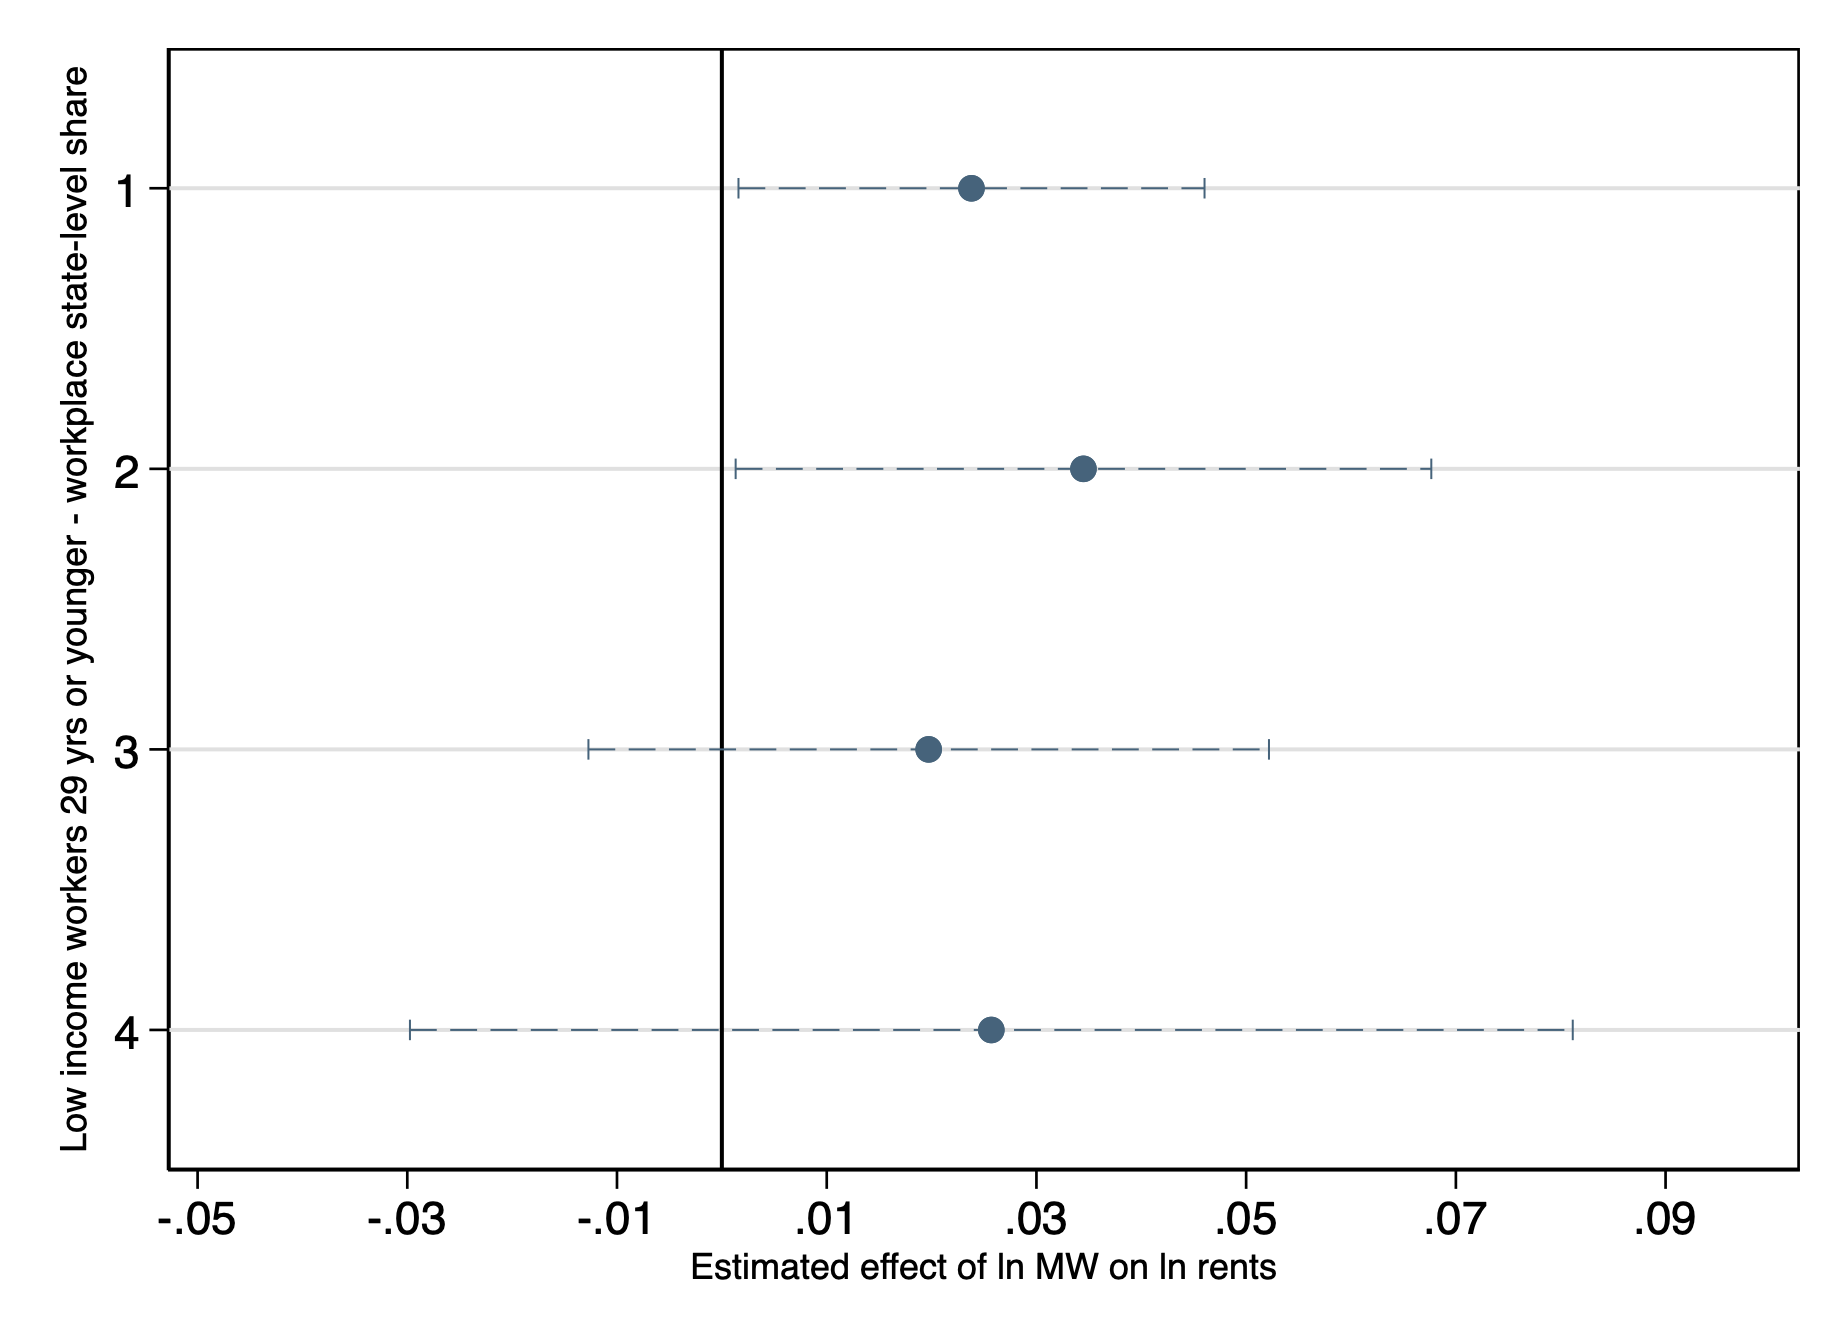
\includegraphics[width = \textwidth]{input/fd_static_heter_walall_29y_lowinc_ssh.png}
    \end{subfigure}
    \begin{subfigure}[b]{0.6\textwidth}
        \caption{Residence location}
        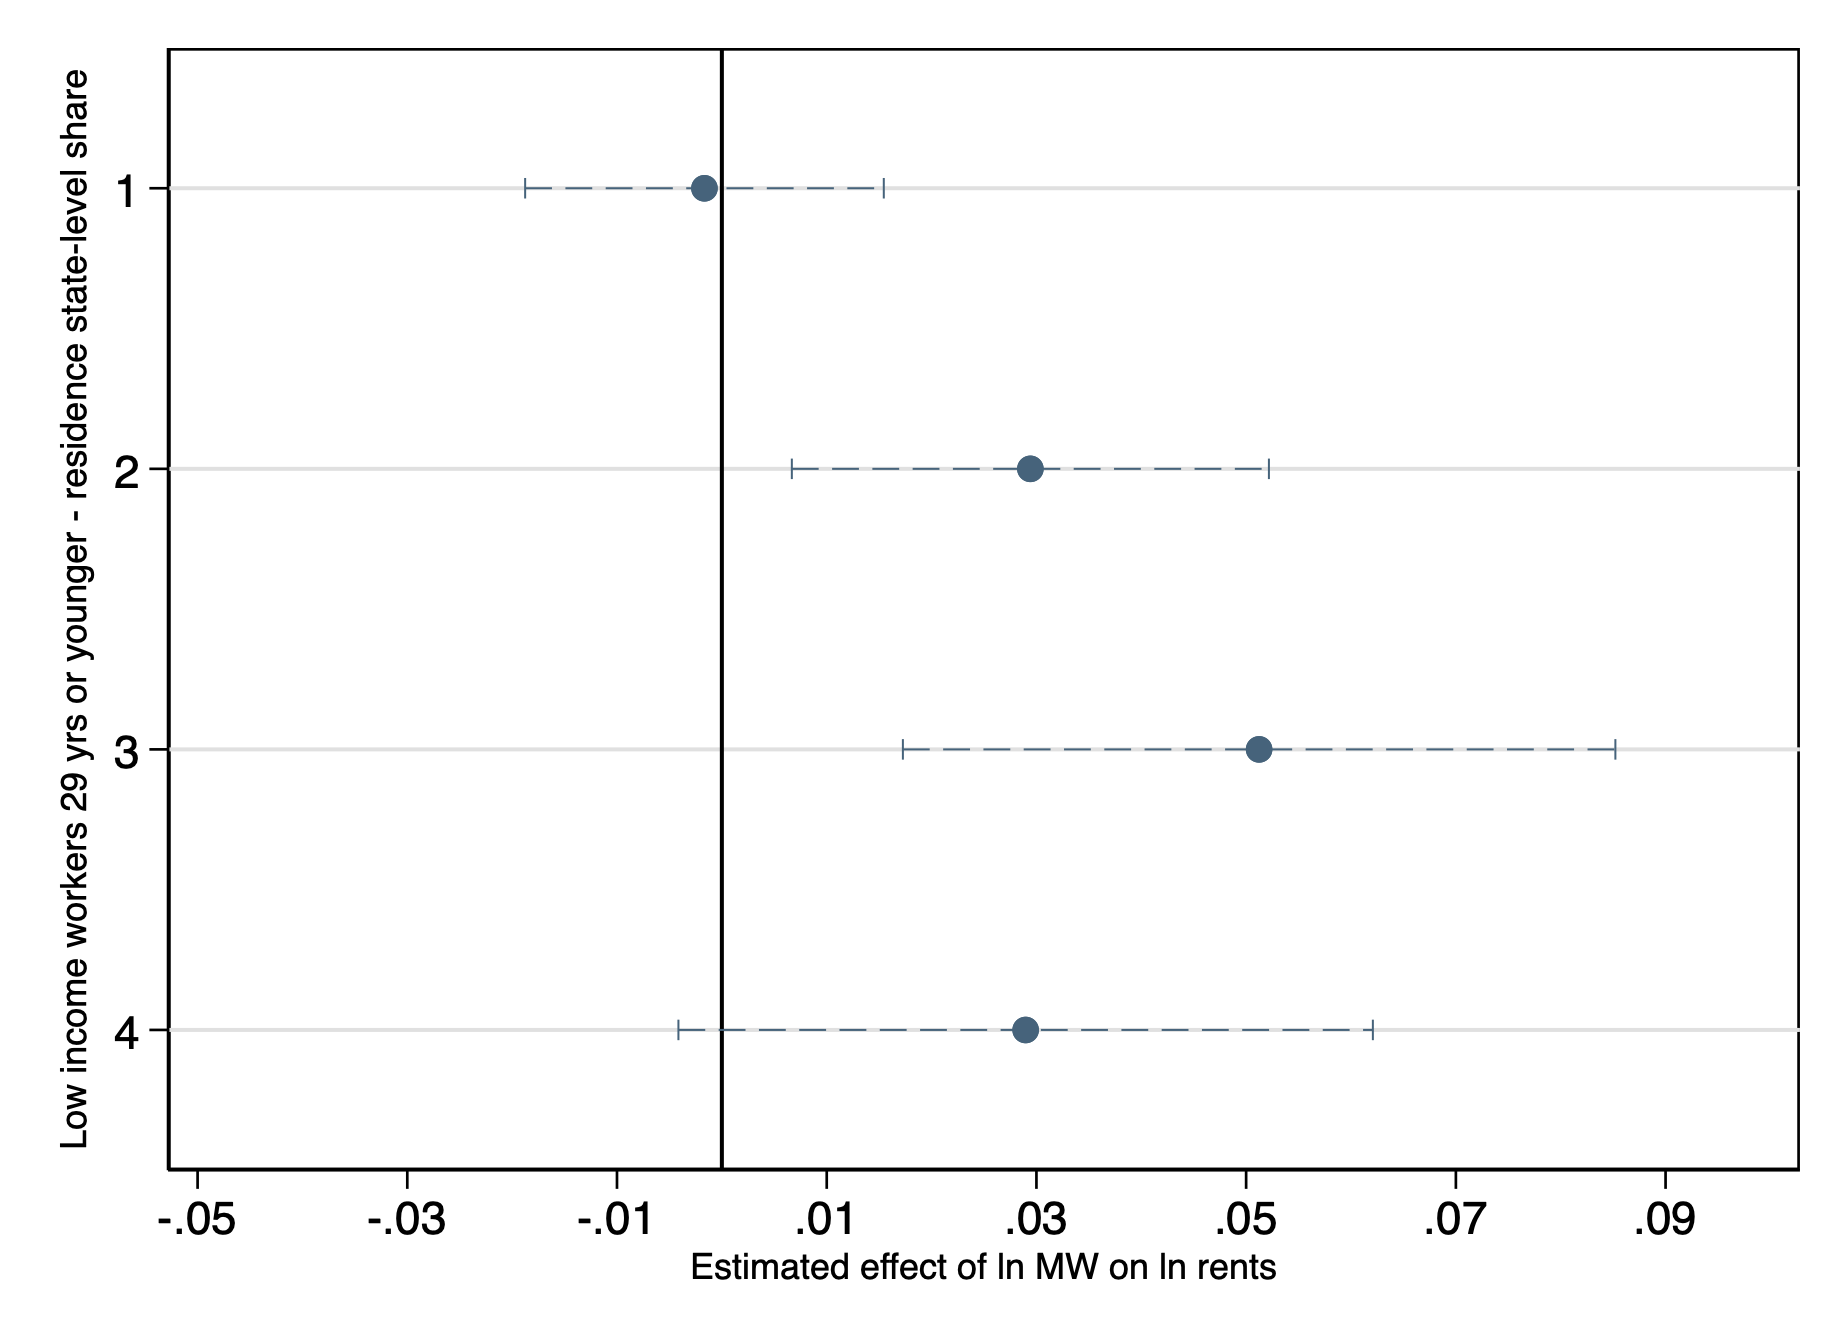
\includegraphics[width = \textwidth]{input/fd_static_heter_halall_29y_lowinc_ssh.png}
    \end{subfigure}
    \begin{minipage}{0.95\textwidth} \footnotesize
		\vspace{2mm} 
		\textit{Notes}: The Figure shows the estimated coefficients $\beta_{q}$, $q \in \{1, 2, 3,
		4\}$ from \autoref{eq:diff_main_hetero} when differentiating zipcodes with respect to the 
		share of MW workers that either work (a) or live (b) in each zipcode. Shares are taken over 
		state totals. MW workers is used as a loose label for workers below 30 years old earning 
		less than $\$1250$ month identified using the 2017 LODES datasets (see \autoref{sec:data} 
		for more information). 90 percent confidence intervals reported.
	\end{minipage}
\end{figure}

In \autoref{fig:static_dd_workers_home_work} we plot the estimated coefficients for the interaction 
between changes in (log) MW and each quartile of the two distributions. Panel (a) presents results 
for MW workplace location. The point estimates are very similar, suggesting that the effect on rents 
is orthogonal to the geographic distribution of MW workplace. The coefficients for the first 2 
quartiles are significant at the $10$ percent level, but standard errors for the $3^{rd}$ and 
$4^{th}$ quartiles become very large partly due to a heavily right-skewed distribution of the 
underlying variable. In panel (b) we re-estimate \autoref{eq:diff_main_hetero} using the MW residence 
distribution. Here we do observe a different pattern: the point estimate in the lowest quartile is 
precisely zero, but this increases and becomes statistically significant both in the $2^{nd}$ and 
$3^{rd}$ quartile. Even more, the effect appears larger: a 10 percent increase in MW leads to a 0.5 
percent increase in rents. The estimated effect for zipcodes with the highest share of young, 
low-income workers decreases to 0.3 percent and becomes not significant, but we notice how also the 
underlying MW residence distribution is heavily right-skewed, and this higher variance partially 
justify the lower precision in our estimates. Overall, this exercise shows how MW workers indeed seem 
to bear most of the impact with relatively higher rents in their place of residence.

The LODES-based proxies for MW workers are approximate by definition. We then turn to investigate 
how the impact of MW changes on rents differs across the distribution for different census-based 
zipcode demographics. The Bureau of Labor Statistics reports how MW workers tend to be young and 
less educated.\footnote{See, for example, BLS Report 1085, \textit{Characteristics of Minimum Wage 
		Workers 2019} at \url{https://www.bls.gov/opub/reports/minimum-wage/2019/home.htm}} 
The study of heterogeneous effects by demographics can therefore help both in confirming what the
LODES-based measures indicate, and in uncovering additional patterns of the effects under study.

\autoref{tab:fd_model_het} shows the estimated coefficients for the interaction between changes in 
(log) MW and quartiles of the distribution for several demographics. In column 1 we show how the 
effect disproportionately impact zipcodes in the lowest quartile of the median income distribution: 
the estimated elasticity of rent to MW is 0.039 (s.e. 0.022). The effect on the other quartiles 
becomes not significant and it shows a non-monotone behavior in the $2^{nd}$ and $3^{rd}$ quartiles. 
When looking at the richest neighborhoods however, we have a markedly smaller and imprecise estimate. 
In column 2 we focus on the zipcode-level unemployment  rate. Not surprisingly, we find that the 
strongest effect is localized in the $4^{th}$ quartile of the distribution, 0.045 (s.e. 0.017). 
Estimates lose significance in the remaining part of the distribution: similarly to column 1, we 
find not-significant not-monotone estimates in the middle quartiles, while the effect is a clear 
zero in the bottom quarter. In column 3 we look at the share of college graduates, and the estimates 
confirm that indeed lower educated neighborhoods bear the bulk of the rent increase: there is a 
clear divide between above median zipcodes showing zero and not significant effects, and below 
median ones where a 10 percent increase in MW leads to a 0.47 and a 0.37 percent rent increase for 
the $2^{nd}$ and $1^{st}$ quartiles, respectively. Lastly, in column 4 we show the impact across 
the distribution over share of African-American residents. Similarly to column 3, we do find a 
stark contrast between above and below median zipcodes. The effect of MW changes on rents 
monotonically increases starting from a not significant effect of 0.017 in the $1^{st}$ quarter to 
a statistically significant 0.042 in the $4^{th}$ one.

\begin{table}[h!]
    \caption{Heterogeneity Results - static DiD model}
    \label{tab:fd_model_het}
    \centering
    \resizebox{0.9\textwidth}{!}{             %%% CHANGE INPUT FOLDER
	    \vspace{0pt}    
	    {
\def\sym#1{\ifmmode^{#1}\else\(^{#1}\)\fi}
\begin{tabular}{l*{6}{c}}
\hline\hline
          &\multicolumn{1}{c}{(1)}&\multicolumn{1}{c}{(2)}&\multicolumn{1}{c}{(3)}&\multicolumn{1}{c}{(4)}&\multicolumn{1}{c}{(5)}&\multicolumn{1}{c}{(6)}\\
          &\multicolumn{1}{c}{\shortstack{Median \\ income}}&\multicolumn{1}{c}{\shortstack{College \\ grad. (\%)}}&\multicolumn{1}{c}{\shortstack{15-24 years \\ old (\%)}}&\multicolumn{1}{c}{\shortstack{African- \\ am. (\%)}}&\multicolumn{1}{c}{\shortstack{Young \\ low-inc. worker,\\ workplace}}&\multicolumn{1}{c}{\shortstack{Young \\ low-inc. worker,\\ residence}}\\
\hline
First quartile&   0.0373         &   0.0356\sym{*}  &   0.0196         &   0.0175         &   0.0214         & -0.00317         \\
          & (0.0223)         & (0.0197)         & (0.0139)         & (0.0159)         & (0.0131)         &(0.00981)         \\
[1em]
Second quartile&   0.0193         &   0.0448\sym{**} &   0.0187         &   0.0217         &   0.0340\sym{*}  &   0.0304\sym{**} \\
          & (0.0146)         & (0.0217)         & (0.0156)         & (0.0157)         & (0.0194)         & (0.0128)         \\
[1em]
Third quartile&   0.0300         &   0.0255         &   0.0212         &   0.0209         &   0.0196         &   0.0498\sym{**} \\
          & (0.0245)         & (0.0208)         & (0.0149)         & (0.0132)         & (0.0187)         & (0.0201)         \\
[1em]
Fourth quartile&   0.0129         &-0.000230         &   0.0414\sym{***}&   0.0404\sym{**} &   0.0249         &   0.0268         \\
          & (0.0126)         & (0.0114)         & (0.0144)         & (0.0162)         & (0.0330)         & (0.0197)         \\
\hline
P-value equality&    0.813         &    0.176         &    0.230         &    0.487         &    0.768         &    0.005         \\
Observations&  107,781         &  107,781         &  107,781         &  107,781         &  107,568         &  107,707         \\
\hline\hline
\end{tabular}
}

    }
    \begin{minipage}{0.95\textwidth} \footnotesize
		\vspace{3mm}
		\textit{Notes}: The table reports estimates for $\beta_{q}$, $q=\{1, 2, 3, 4\}$ from 
		\autoref{eq:diff_main_hetero} when differentiating zipcodes based on several 
		socio-demographics from the 2010 Census and the 5-year 2008-2012 ACS. Standard errors 
		clustered at the state level. *** $p < 0.01$, ** $p < 0.05$, * $p < 0.1$.  
	\end{minipage}
\end{table}
